\documentclass[paper=a4, fontsize=11pt]{scrartcl}
\usepackage[T1]{fontenc}  % proper encoding for output file
\usepackage[utf8]{inputenc}  % except UTF-8 character in source
\usepackage[english]{babel}  % set document language
\usepackage{amsmath,amsfonts,amsthm}  % math type setting
\usepackage{mhchem}  % chemical expressions
\usepackage{graphicx}  % inclue graphics
\usepackage{url}
\usepackage{caption}
\usepackage{subcaption}
\setlength\parindent{0pt} % Removes all indentation from paragraphs


\title{Exercise 1: Rotational Spectra}
\author{Sample Solution}
\date{Effective: 19.10.2016}

%%%%%%%%%%%%%%%%%%%%%%%%%%%%%%%%%%%%%%%%%%%%%%%%%%%%%%%%%%%%%%%%%%%%%%%%%%%%%%%
\begin{document}

\maketitle

1. Calculate the absorption cross sections in the microwave spectral range for the
following molecules:
\begin{itemize}
    \item $HCl$
    \item $ClO$
    \item $CO$
    \item $N_2O$
    \item $O_3$
\end{itemize}
Unless otherwise specified use the parameter setting as given in the example
file \path{absorption.arts}.

% figures abs cross sections
\begin{figure}[t!]
    \centering
    \begin{subfigure}[t]{0.45\textwidth}
        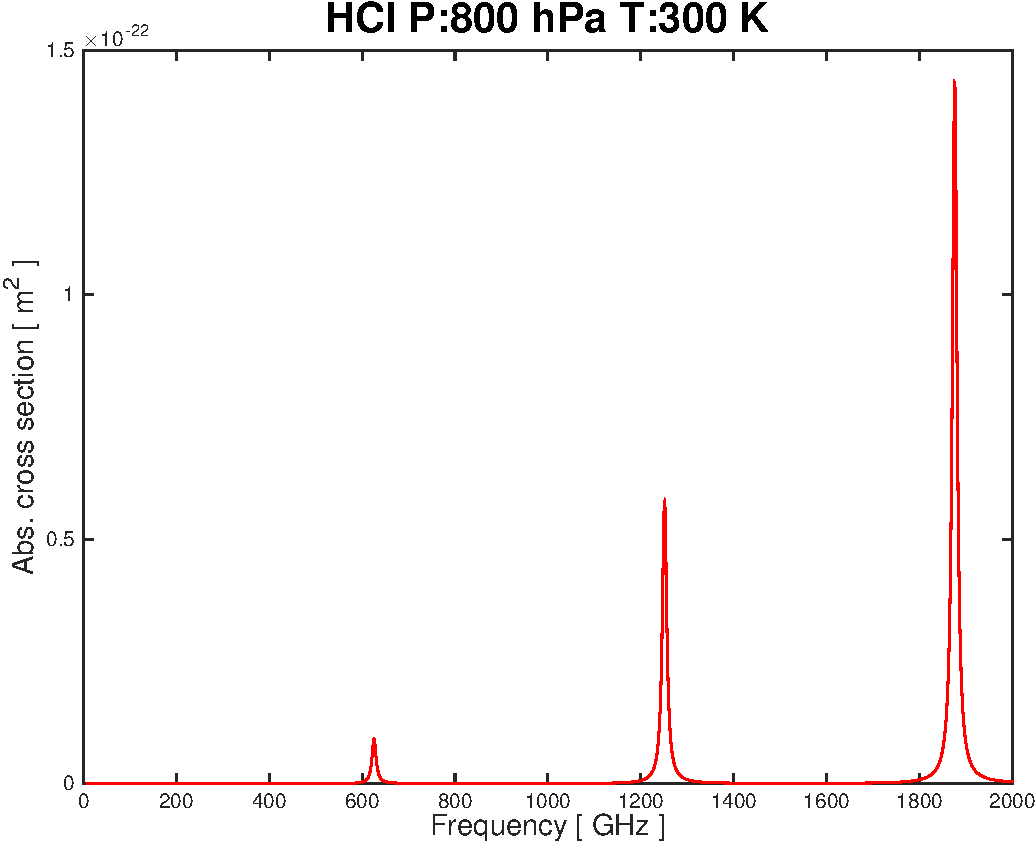
\includegraphics[width=\textwidth]{plots/plot_xsec_HCl_800hPa_300K.pdf}
        \caption{HCl}
    \end{subfigure}
    \begin{subfigure}[t]{0.45\textwidth}
        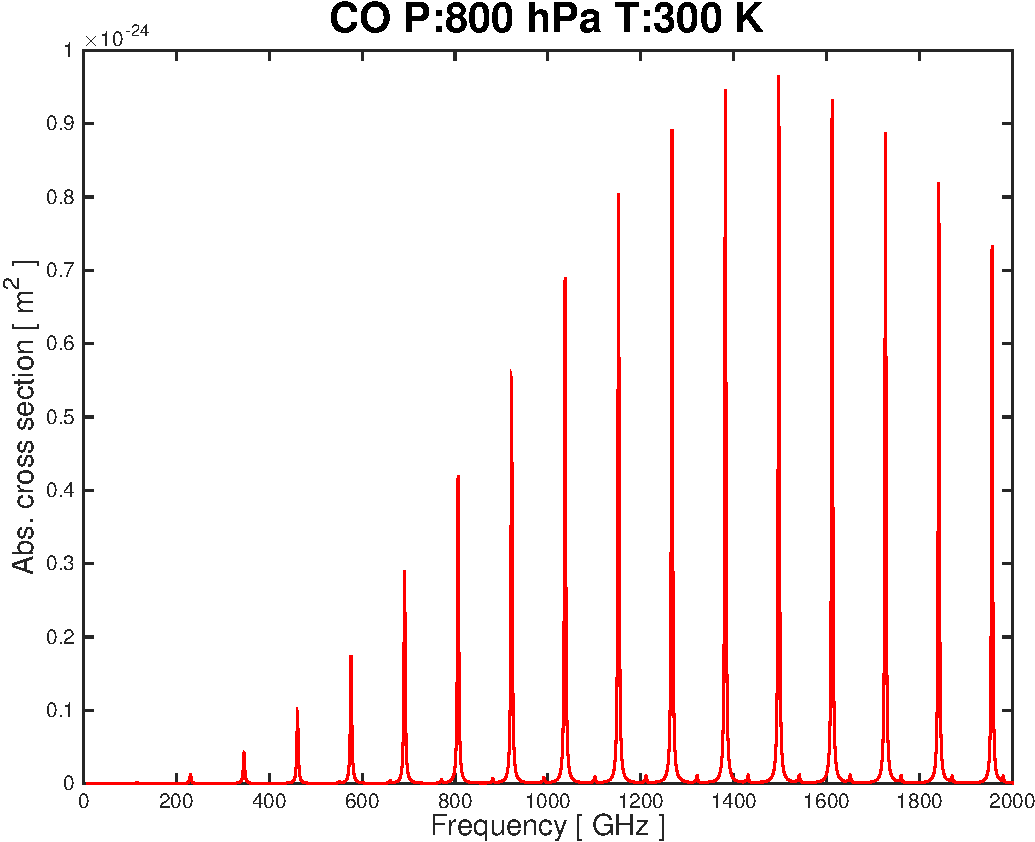
\includegraphics[width=\textwidth]{plots/plot_xsec_CO_800hPa_300K.pdf}
        \caption{$CO$}
    \end{subfigure}
    \begin{subfigure}[b]{0.45\textwidth}
        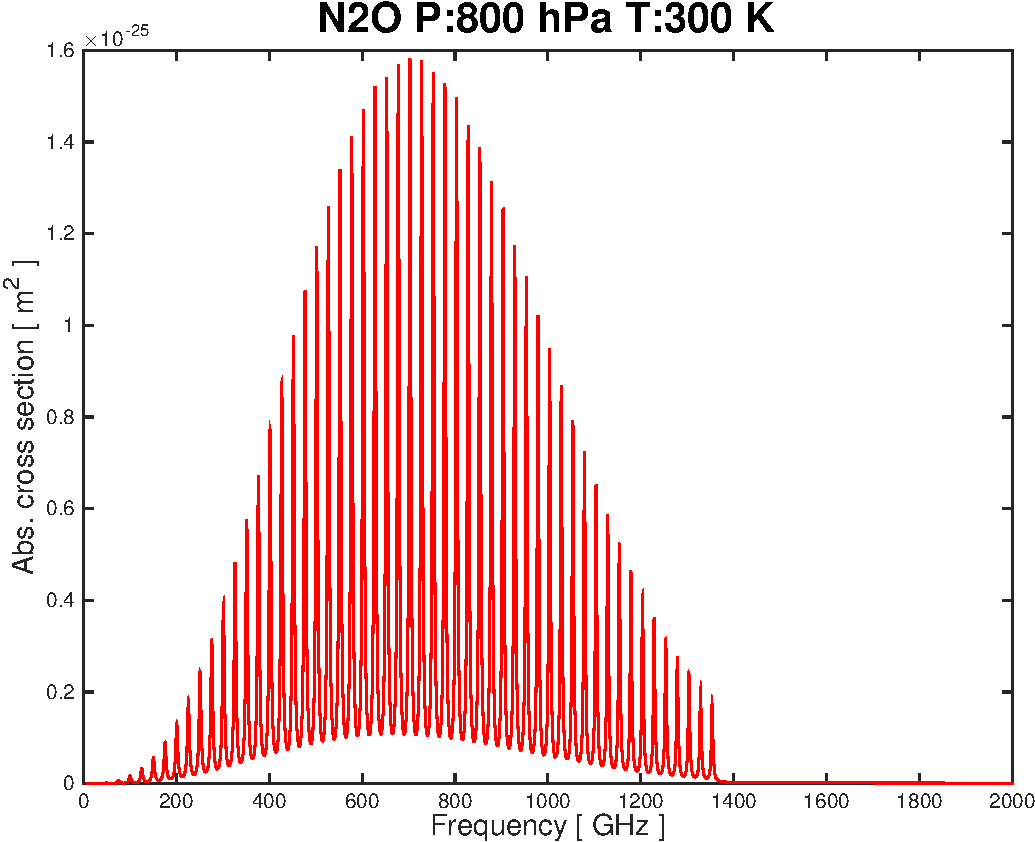
\includegraphics[width=\textwidth]{plots/plot_xsec_N2O_800hPa_300K.pdf}
        \caption{$N_2O$}
    \end{subfigure}
    \begin{subfigure}[b]{0.45\textwidth}
        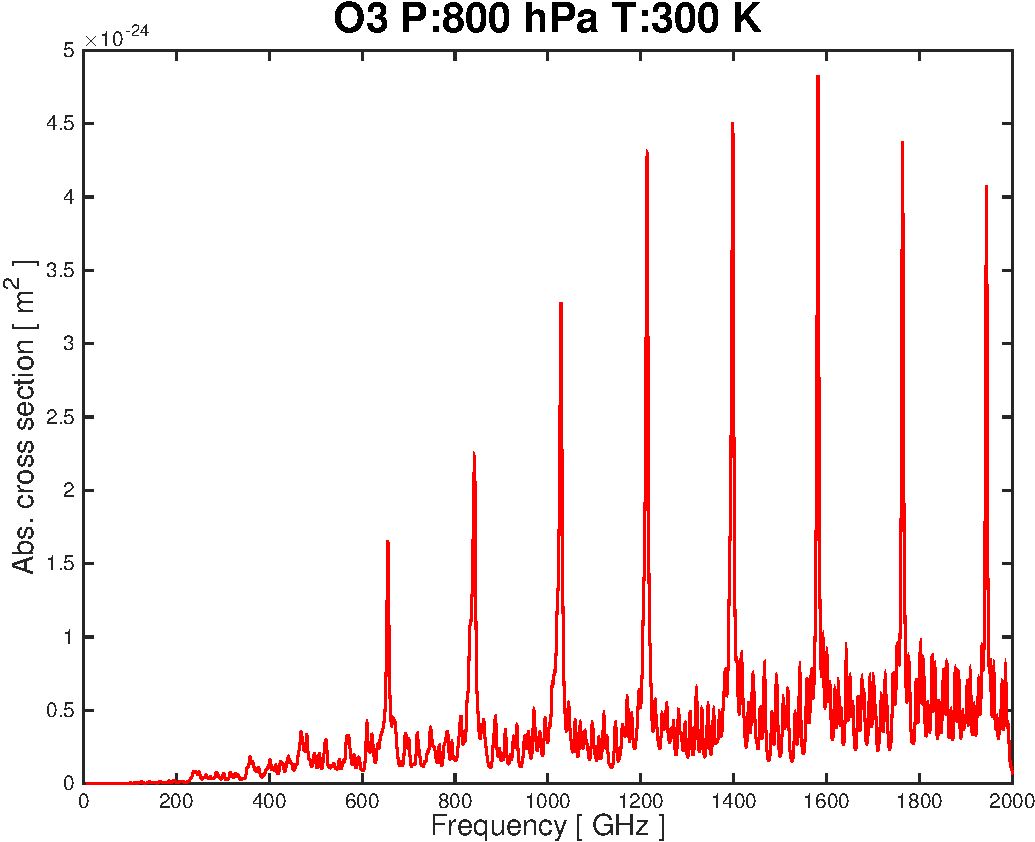
\includegraphics[width=\textwidth]{plots/plot_xsec_O3_800hPa_300K.pdf}
        \caption{$O_3$}
    \end{subfigure}
    \begin{subfigure}[b]{0.45\textwidth}
        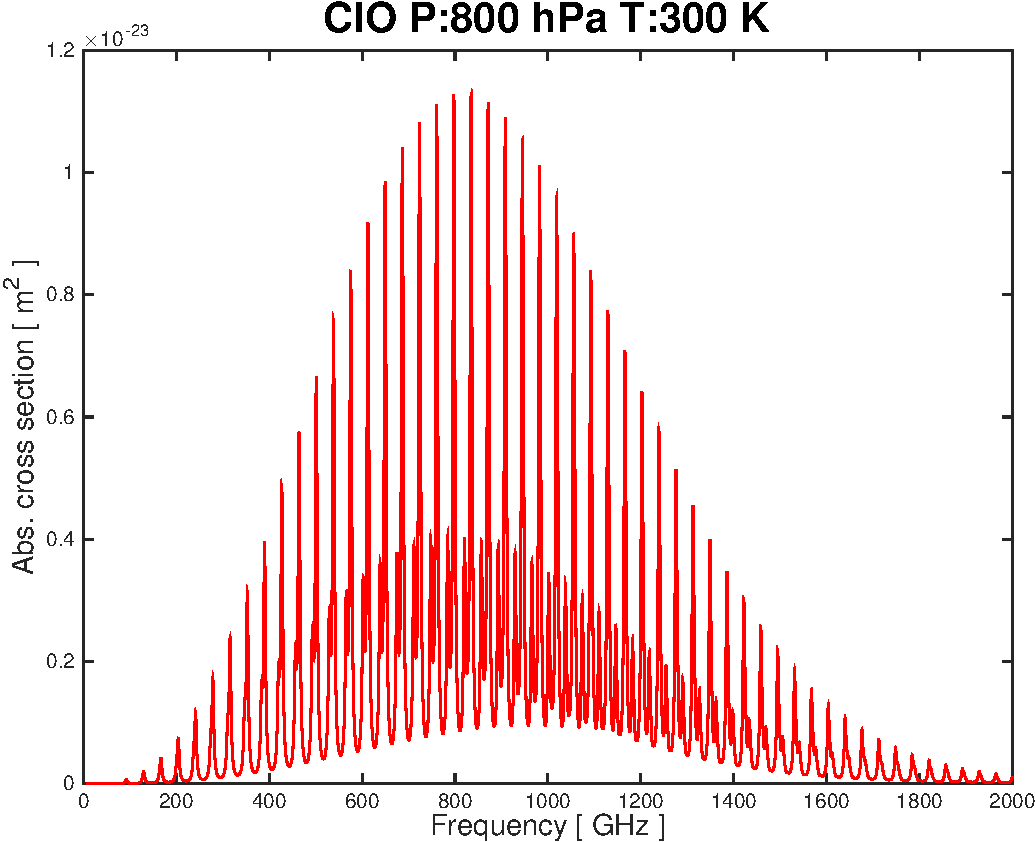
\includegraphics[width=\textwidth]{plots/plot_xsec_ClO_800hPa_300K.pdf}
        \caption{$ClO$}
    \end{subfigure}

    \caption{Absorption cross sections of the molecules $HCl$, $ClO$, $CO$,
    $N_2O$ and $O_3$.}
    \label{fig:abs_molecules}
\end{figure}

\begin{itemize}
    \item Estimate the rotational constant $B$ for $HCl$ and for $CO$.
    \begin{itemize}
        \item $B_{HCl} \approx 300$\,GHz
        \item $B_{CO} \approx 100$\,GHz
    \end{itemize}
    \item Why is B larger for $HCl$ than for $CO$?
    \begin{itemize}
        \item The reduced mass $\mu$ is larger for $HCl$. This is caused by a
            larger molecule in general and a larger mass difference of the
            atoms inside the molecule.
    \end{itemize}
    \item Do you have any idea why $N_{2}O$ behaves like a diatomic molecule -
        and $O_{3}$ not?
    \begin{itemize}
        \item The angles between the atoms inside the molecule differ. $N_2O$
            has flat angles and therefore momentums of inertia like a linear
            molecule ($I_A = 0, I_B = I_C$). $O_3$ has a more complex structure
            with differing momentums of inertia ($I_A \neq I_B \neq I_C$).
    \end{itemize}
\end{itemize}

2. Investigate other molecules!

\clearpage
3. Show for a diatomic molecule that the moment of inertia is given by $I = \mu r_0^2$.
\begin{equation*}
  I = \sum_i m_i r_i^2 = m_1 r_1^2 + m_2 r_2^2
\end{equation*}
The center of gravity is defined as $m_1 r_1 = m_2 r_2$. Insert this and you get
\begin{align}
  I &= m_2 r_2 r_1 + m_1 r_1 r_2 \nonumber\\
    &= r_1 r_2 (m_1 + m_2) \label{eq:a}
\end{align}
We can do more with the center of gravity equation:
\begin{align}
  m_1 r_1 &= m_2 r_2 = m_2 \overbrace{(r_0 - r_1)}^\text{from def.} = m_2 r_0 - m_2 r_1 \nonumber\\
  (m_1 + m_2) r_1 &= m_2 r_0 \nonumber\\
  r_1 &= \frac{m_2 r_0}{m_1 + m_2} \label{eq:b}\\
  r_2 &= \frac{m_1 r_0}{m_1 + m_2} \label{eq:c}
\end{align}
Insert (\ref{eq:b}) and (\ref{eq:c}) into (\ref{eq:a}):
\begin{align*}
  I &= \frac{m_2r_0 \; m_1r_0 \; (m_1 + m_2)}{(m_1 + m_2)(m_1 + m_2)} \\
    &= \frac{m_1m_2}{m_1 + m_2} r_0^2 = \mu r_0^2 \qquad\square
\end{align*}
\end{document}
